\iffalse
\let\negmedspace\undefined
\let\negthickspace\undefined
\documentclass[journal,12pt,twocolumn]{IEEEtran}
\usepackage{cite}
\usepackage{amsmath,amssymb,amsfonts,amsthm}
\usepackage{algorithmic}
\usepackage{graphicx}
\usepackage{textcomp}
\usepackage{xcolor}
\usepackage{txfonts}
\usepackage{listings}
\usepackage{enumitem}
\usepackage{mathtools}
\usepackage{gensymb}
\usepackage{comment}
\usepackage[breaklinks=true]{hyperref}
\usepackage{tkz-euclide} 
\usepackage{listings}
\usepackage{gvv}                                        
\def\inputGnumericTable{}                                 
\usepackage[latin1]{inputenc}                                
\usepackage{color}                                            
\usepackage{array}                                            
\usepackage{longtable}                                       
\usepackage{calc}                                             
\usepackage{multirow}                                         
\usepackage{hhline}                                           
\usepackage{ifthen}                                           
\usepackage{lscape}
\usepackage{placeins}
\usepackage{xparse}


\newtheorem{theorem}{Theorem}[section]
\newtheorem{problem}{Problem}
\newtheorem{proposition}{Proposition}[section]
\newtheorem{lemma}{Lemma}[section]
\newtheorem{corollary}[theorem]{Corollary}
\newtheorem{example}{Example}[section]
\newtheorem{definition}[problem]{Definition}
\newcommand{\BEQA}{\begin{eqnarray}}
\newcommand{\EEQA}{\end{eqnarray}}
\newcommand{\define}{\stackrel{\triangle}{=}}
\theoremstyle{remark}
\newtheorem{rem}{Remark}

\graphicspath{ {./figs/} } 

\begin{document}

\bibliographystyle{IEEEtran}
\vspace{3cm}

\Large\title{GATE 2021 EC 5}
\large\author{EE23BTECH11032 - Kaustubh Parag Khachane $^{*}$% <-this % stops a space
}
\maketitle
\newpage
\bigskip

\renewcommand{\thefigure}{\theenumi}
\renewcommand{\thetable}{\theenumi}
\large\textbf{Question GATE 21 EC 5} :\\
Consider two 16-point sequences x\sbrak{n} and h\sbrak{n}. Let the linear convolution of x\sbrak{n} and h\sbrak{n} be denoted by y\sbrak{n}, while z\sbrak{n} denotes the 16-point inverse discrete Fourier transform \brak{IDFT} of the product of the 16-point DFTs of x\brak{n} and h\sbrak{n}. The values of k for which z\sbrak{k} = y\sbrak{k} are 
\begin{enumerate}
    \item $k = 0, 1, 2, 3, ... , 15$
    \item $k = 0$
    \item $k = 15$
    \item $k = 0$ and $k = 15$
\end{enumerate}
\hfill(GATE EC 2021)\\
\solution\\
\fi
\begin{table}[!ht] 
\centering
\setlength{\extrarowheight}{8pt}
\begin{tabular}{|l|l|}
    \hline
    \textbf{Parameter} & \textbf{Description}  \\\hline
     x\sbrak{n} & Given 16 point sequence \\\hline
     h\sbrak{n} &  Given 16 point sequence \\\hline
     y\sbrak{n} & Linear convolution of x\sbrak{n} and h\sbrak{n} \\\hline
     z\sbrak{n} & IDFT of products of DFTs of h\sbrak{n} and x\sbrak{n} \\\hline
     N & number of terms \brak{16} \\\hline
    \end{tabular}
  \vspace{4mm}
 \caption{Parameter Table}
 \label{tab:table0_ec5}
\end{table}

We can write z\sbrak{n} as ,
\begin{align}
    z\sbrak{n} = IDFT\sbrak{X\sbrak{f}H\sbrak{f}}
\end{align}
We know that product in frequency domain is convolution in time domain. However, z\sbrak{n} is not linear convolution of x\sbrak{n} and h\sbrak{n} in the time domain due to periodicity of DFT. Point-wise multiplication in the frequency domain (product of DFTs) doesn't translate directly to convolution in the time domain due to periodicity and potential aliasing.\\
z\sbrak{n} is the circular convolution of x\sbrak{n} and h\sbrak{n}. Using the formula for circular convolution,
\begin{align}
    z\sbrak{n} = \sum_{m = -\infty}^{\infty}\brak{h\sbrak{m} \sum_{p = -\infty}^{\infty}x\sbrak{n - m -pN}} \label{eq:eq1_g21ec5}
\end{align}
y\sbrak{n} is a linear convolution of x\sbrak{n} and h\sbrak{n}.
\begin{align}
    y\sbrak{n} = \sum_{m = -\infty}^{\infty} x\brak{m} h\sbrak{n-m}
\end{align}
Each term of y\sbrak{n} will be sum of products of terms of x\sbrak{n} and h\sbrak{n}. The number of terms in each summation will go from 1 for $n=1$ to 16 for $n=15$. \\
z\sbrak{n} is expressed as sum of 15 terms for all permissible values of n using $p=0$ or $p=1$ in \eqref{eq:eq1_g21ec5}.
\\ Thus,$z\sbrak{k} = y\sbrak{k}$ can be possible for only $k=15$.
\\ For $k = 15$,
\begin{align}
    y\sbrak{15} &= x\sbrak{0}h\sbrak{15} +  x\sbrak{1}h\sbrak{14} + ...  x\sbrak{15}h\sbrak{0} 
\end{align}
Using p = 0  in \eqref{eq:eq1_g21ec5},
\begin{align}
    z\sbrak{15} &= h\sbrak{0} x\sbrak{15} + h\sbrak{1} x\sbrak{14} + ... h\sbrak{15} x\sbrak{0}\\
    &=  x\sbrak{0}h\sbrak{15} +  x\sbrak{1}h\sbrak{14} + ...  x\sbrak{15}h\sbrak{0} 
\end{align}
Thus , z\sbrak{15} = y\sbrak{15}.\\
Graphically, let 
\begin{align}
    x &= \sbrak{1,2,3,4,....,16}\\
    h &= \sbrak{1,1,1,1, ... 1}
\end{align}
Then the plot for z and y is as shown bellow.
\begin{figure}[!ht]
\centering
\begin{center}
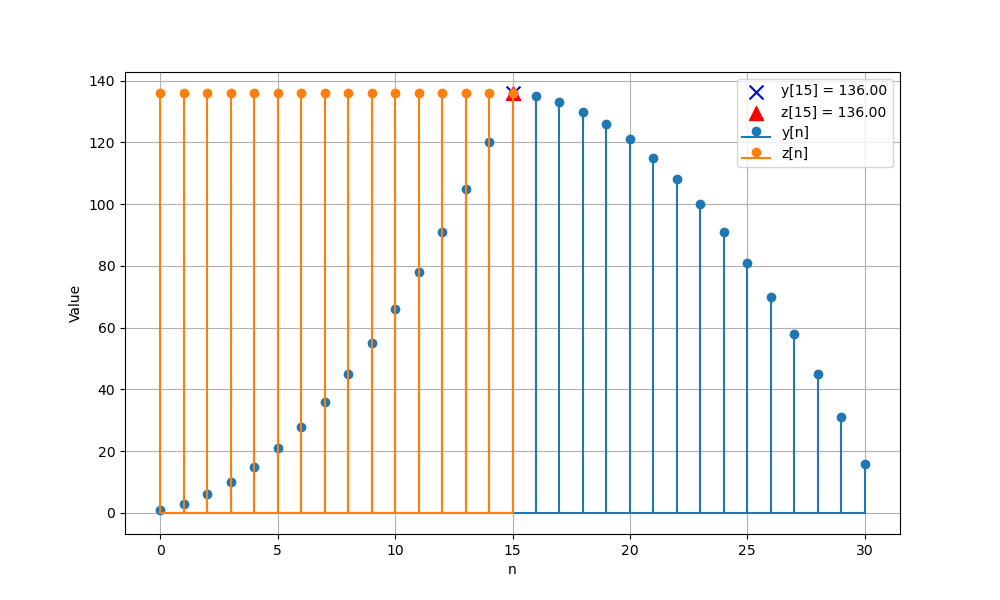
\includegraphics[width=\columnwidth]{2021/EC/5/figs/Figure_1.png}
\end{center}
\caption{Plot of y\sbrak{n} and z\sbrak{n}}
\end{figure}
